\scanpage{293}

$\begin{pmatrix}\lambda&0\\0&\lambda^{-1}\end{pmatrix}$ normalisa\unsure{teur|tion} de $U_0$ opère sur $U_0$, par $\boxed{\lambda^2}$

et $\lambda:\mathrm{Et}(s)\xrightarrow{\sim}\mathrm{Et}(\lambda^{-1}s)$ qui transforme $\omega_s$ pour une orientation fixée en $\omega_{\lambda^{-1}s}^{\boxed{\lambda^2}}$ i.e.

\[
\boxed{\lambda\cdot(a\dotplus\zeta)=\lambda a+\lambda^2\zeta}
\]

Donc on ne récupère là que $\lambda^2$, pas $\lambda$ ! Mais la relation d'incidence entre $a\underset{s}{\dotplus}\zeta\in\mathrm{Et}(s)$ et $\lambda a\underset{\lambda^{-1}s}{\dotplus}\zeta'$ est

\[
\deleted{a}\quad\zeta'=\lambda^2\zeta\pm\lambda
\]

i.e. les quantités $\zeta'-\underset{\text{\uline{connu}}}{\underline{\lambda^2}}\zeta$ forment \unsure{l'ens|l'ens.|l'élém.} $\{\pm\lambda\}$ !

\noindent\rule{\linewidth}{.35pt}

\[
\zeta,\zeta'\ \text{incidents}\qquad\zeta'=\pm\lambda\qquad\deleted{\lambda\zeta}\qquad t'\pm\unsure{\nu|v}_{\lambda}
\]

\figure{\begin{tikzpicture}[x=.84cm,y=.84cm]
\draw (0,0)--(1.57,.37) (1.72,.07)--(3.25,.07) (3.42,.20)--(4.75,-.27);
\foreach \x/\y in {0/0,1.57/.37,3.18/.36}{\fill (\x,\y) circle (1.3pt);}
\node[below] at (0,0) {$s$};\node[above] at (1.57,.37) {$t$};\node[above right] at (3.18,.36) {$\lambda t=t'$};
\node at (1.75,.07) {$\deleted{a}$};\node at (3.15,.07) {$\deleted{\lambda a}$};
\node[right] at (4.75,-.27) {$\lambda^{-1}s=s'$};
\draw[very thin] (3.34,.22)..controls (1.09,-2.83) and (6.90,-4.41)..(8.16,-1.91)
..controls (9.40,.59) and (7.78,-.3)..(8.15,.12)
..controls (8.39,3.13) and (5.3,3.47)..(3.34,.22);
\node[right] at (8.62,1.0) {$\deleted{\unsure{a_0}}$};
\end{tikzpicture}}

\margin{$\mu(\lambda)$}

\figure{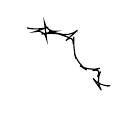
\begin{tikzpicture}[x=0.008cm,y=-0.008cm]
\draw[rounded corners] (0,0)--(15,4)--(27,0)--(28,8)--(38,6)--(50,9)--(65,15)--(73,8)--(71,31)--(78,57)--(97,69)--(119,62)--(106,84)--(113,94)--(125,92);
\end{tikzpicture}}

\[
\begin{aligned}
\zeta'_1&=\lambda^2\zeta+\lambda & \left\{\begin{aligned}\zeta'_1+\zeta'_2&=2\lambda^2\zeta\\\zeta'_1-\zeta'_2&=2\lambda\end{aligned}\right.\\[-1.8ex]
\zeta'_2&=\lambda^2\zeta-\lambda
\end{aligned}
\]

\[
\boxed{\underset{\substack{\rotatebox{90}{$\in$}\\\mathrm{Et}(s)}}{a}\ \text{incident :}\quad \lambda(a)\underset{\lambda^{-1}(s)}{\overset{\cdot}{\pm}}\underset{\substack{\rotatebox{90}{$\in$}\\\Lambda}}{\lambda}}
\]

\figure{\begin{tikzpicture}[x=0.008cm,y=-0.008cm]
\draw (0,0)--(162,-9);
\node[right] at (162,-9) {$s'$};
\end{tikzpicture}}

% archive sheet number: 292
